\documentclass[12pt,spanish,fleqn,openany,pagesize]{report}%{scrbook}

\usepackage[utf8]{inputenc}
\usepackage[spanish]{babel}
\usepackage{fancyhdr}
\usepackage{epsfig}
\usepackage{epic}
\usepackage{eepic}
\usepackage{amsmath}
\usepackage{threeparttable}
\usepackage{amscd}
\usepackage{here}
\usepackage{graphicx}
\usepackage{lscape}
\usepackage{tabularx}
\usepackage{subfigure}
\usepackage{longtable}
\usepackage[table,xcdraw]{xcolor}
\usepackage{times}
\usepackage{url}
\usepackage{color}   %May be necessary if you want to color links
\usepackage{titlesec}
\usepackage{hyperref}
\usepackage[resetlabels,labeled]{multibib}
\usepackage{enumitem}
\usepackage{listings}

\newcites{W}{Referencias Web}

\hypersetup{
    colorlinks=false, %set true if you want colored links
    linktoc=all,     %set to all if you want both sections and subsections linked
    linkcolor=blue,  %choose some color if you want links to stand out
}
\pagenumbering{arabic}

\usepackage{rotating} %Para rotar texto, objetos y tablas seite. No se ve en DVI solo en PS. Seite 328 Hundebuch
                        %se usa junto con \rotate, \sidewidestable ....



\titleclass{\subsubsubsection}{straight}[\subsection]

\newcounter{subsubsubsection}[subsubsection]
\renewcommand\thesubsubsubsection{\thesubsubsection.\arabic{subsubsubsection}}
\renewcommand\theparagraph{\thesubsubsubsection.\arabic{paragraph}} % optional; useful if paragraphs are to be numbered

\titleformat{\subsubsubsection}
  {\normalfont\normalsize\bfseries}{\thesubsubsubsection}{1em}{}
\titlespacing*{\subsubsubsection}
{0pt}{3.25ex plus 1ex minus .2ex}{1.5ex plus .2ex}

\makeatletter
\renewcommand\paragraph{\@startsection{paragraph}{5}{\z@}%
  {3.25ex \@plus1ex \@minus.2ex}%
  {-1em}%
  {\normalfont\normalsize\bfseries}}
\renewcommand\subparagraph{\@startsection{subparagraph}{6}{\parindent}%
  {3.25ex \@plus1ex \@minus .2ex}%
  {-1em}%
  {\normalfont\normalsize\bfseries}}
\def\toclevel@subsubsubsection{4}
\def\toclevel@paragraph{5}
\def\toclevel@paragraph{6}
\def\l@subsubsubsection{\@dottedtocline{4}{7em}{4em}}
\def\l@paragraph{\@dottedtocline{5}{10em}{5em}}
\def\l@subparagraph{\@dottedtocline{6}{14em}{6em}}
\makeatother





\renewcommand{\theequation}{\thechapter-\arabic{equation}}
\renewcommand{\thefigure}{\textbf{\thechapter-\arabic{figure}}}
\renewcommand{\thetable}{\textbf{\thechapter-\arabic{table}}}


\pagestyle{fancyplain}%\addtolength{\headwidth}{\marginparwidth}
\textheight22.5cm \topmargin0cm \textwidth16.5cm
\oddsidemargin0.5cm \evensidemargin-0.5cm%
\renewcommand{\chaptermark}[1]{\markboth{\thechapter\; #1}{}}
\renewcommand{\sectionmark}[1]{\markright{\thesection\; #1}}
\lhead[\fancyplain{}{\thepage}]{\fancyplain{}{\rightmark}}
\rhead[\fancyplain{}{\leftmark}]{\fancyplain{}{\thepage}}
\fancyfoot{}
\thispagestyle{fancy}%


\addtolength{\headwidth}{0cm}
\unitlength1mm %Define la unidad LE para Figuras
\mathindent0cm %Define la distancia de las formulas al texto,  fleqn las descentra
\marginparwidth0cm
\parindent0cm %Define la distancia de la primera linea de un parrafo a la margen

%Para tablas,  redefine el backschlash en tablas donde se define la posici\'{o}n del texto en las
%casillas (con \centering \raggedright o \raggedleft)
\newcommand{\PreserveBackslash}[1]{\let\temp=\\#1\let\\=\temp}
\let\PBS=\PreserveBackslash

%Espacio entre lineas
\renewcommand{\baselinestretch}{1.1}

%Neuer Befehl f\"{u}r die Tabelle Eigenschaften der Aktivkohlen
\newcommand{\arr}[1]{\raisebox{1.5ex}[0cm][0cm]{#1}}

%Neue Kommandos
\usepackage{Befehle}


%Trennungsliste
\hyphenation {Reaktor-ab-me-ssun-gen Gas-zu-sa-mmen-set-zung
Raum-gesch-win-dig-keit Durch-fluss Stick-stoff-gemisch
Ad-sorp-tions-tem-pe-ra-tur Klein-schmidt
Kohlen-stoff-Mole-kular-siebe Py-rolysat-aus-beu-te
Trans-port-vor-gan-ge}


\definecolor{mygreen}{rgb}{0,0.6,0}
\definecolor{mygray}{rgb}{0.5,0.5,0.5}
\definecolor{mymauve}{rgb}{0.58,0,0.82}

\lstset{ 
  backgroundcolor=\color{white},   % choose the background color; you must add \usepackage{color} or \usepackage{xcolor}; should come as last argument
  basicstyle=\footnotesize,        % the size of the fonts that are used for the code
  breakatwhitespace=false,         % sets if automatic breaks should only happen at whitespace
  breaklines=true,                 % sets automatic line breaking
  captionpos=b,                    % sets the caption-position to bottom
  commentstyle=\color{mygreen},    % comment style
  deletekeywords={...},            % if you want to delete keywords from the given language
  escapeinside={\%*}{*)},          % if you want to add LaTeX within your code
  extendedchars=true,              % lets you use non-ASCII characters; for 8-bits encodings only, does not work with UTF-8
  firstnumber=1000,                % start line enumeration with line 1000
  frame=single,	                   % adds a frame around the code
  keepspaces=true,                 % keeps spaces in text, useful for keeping indentation of code (possibly needs columns=flexible)
  keywordstyle=\color{blue},       % keyword style
  language=Octave,                 % the language of the code
  morekeywords={*,...},            % if you want to add more keywords to the set
  numbers=left,                    % where to put the line-numbers; possible values are (none, left, right)
  numbersep=5pt,                   % how far the line-numbers are from the code
  numberstyle=\tiny\color{mygray}, % the style that is used for the line-numbers
  rulecolor=\color{black},         % if not set, the frame-color may be changed on line-breaks within not-black text (e.g. comments (green here))
  showspaces=false,                % show spaces everywhere adding particular underscores; it overrides 'showstringspaces'
  showstringspaces=false,          % underline spaces within strings only
  showtabs=false,                  % show tabs within strings adding particular underscores
  stepnumber=2,                    % the step between two line-numbers. If it's 1, each line will be numbered
  stringstyle=\color{mymauve},     % string literal style
  tabsize=2,	                   % sets default tabsize to 2 spaces
  title=\lstname                   % show the filename of files included with \lstinputlisting; also try caption instead of title
}

%\includeonly{Kap1/Kap1,Kap2/Kap2}
\begin{document}
%\newpage
%\setcounter{page}{1}
\begin{center}
\begin{figure}
\centering%

\epsfig{file=HojaTitulo/Logoud.png,scale=0.4}%
\end{figure}
\thispagestyle{empty} \vspace*{0.5cm} \textbf{ \LARGE
CREACIÓN DE UN PROTOTIPO DE APLICACIÓN MÓVIL EN 
DISPOSITIVOS ANDROID PARA LA CONTRATACIÓN Y PROMOCIÓN DE MÚSICOS 
}\\[3.5cm]
\Large\textbf{Gustavo Alejandro Realpe Fresneda}\\
\Large\textbf{David Fernando Cabarcas Bolaños}\\[4.5cm]
\small Universidad Distrital Francisco Jos\'{e} de Caldas\\
Especialización en Ingeniería de Software\\
Bogotá, Colombia\\
A\~{n}o \the\year\\
\end{center}

%\newpage
%\setcounter{page}{1}
\begin{center}
\begin{figure}
\centering%

\epsfig{file=HojaTitulo/Logoud.png,scale=0.4}%
\end{figure}
\thispagestyle{empty}  \textbf{ \LARGE
CREACIÓN DE UN PROTOTIPO DE APLICACIÓN MÓVIL EN 
DISPOSITIVOS ANDROID PARA LA CONTRATACIÓN Y PROMOCIÓN DE MÚSICOS 
}\\[2cm]
\Large\textbf{Gustavo Alejandro Realpe Fresneda}\\
\Large\textbf{David Fernando Cabarcas Bolaños}\\[2.0cm]

\large\textbf{Director: Giovanny Tarazona}\\
\large\textbf{Revisor: Julio Baron Velandia}\\[3.5cm]


\small Universidad Distrital Francisco Jos\'{e} de Caldas\\
Especialización en Ingeniería de Software\\
Bogotá, Colombia\\
A\~{n}o \the\year\\
\end{center}


\renewcommand{\tablename}{\textbf{Tabla}}
\renewcommand{\figurename}{\textbf{Figura}}
\renewcommand{\listtablename}{Lista de Tablas}
\renewcommand{\listfigurename}{Lista de Figuras}
\renewcommand{\contentsname}{Contenido}


%\newcommand{\clearemptydoublepage}{\newpage{\pagestyle{empty}\cleardoublepage}}
\tableofcontents
%\include{Resumen}
%\newcommand{\clearemptydoublepage}{\newpage{\pagestyle{empty}\cleardoublepage}}
\setcounter{page}{1}
\chapter*{INTRODUCCIÓN}
\addcontentsline{toc}{chapter}{INTRODUCCIÓN}  
La realización de este proyecto supone un fondo social en el que se busca facilitar y mejorar la calidad de vida de las personas dedicadas a la prestación de servicios de entretenimiento que no tienen un conocimiento administrativo o de mercadeo adecuado para promocionar esta labor. Lo anterior toma mayor valor teniendo en cuenta la amplia oferta de programas educativos en programas universitario de música y arte que están produciendo gran número de egresados, que no encontrarán una demanda laboral favorable y se perderán en un mercado hostil que probablemente los llevará a desempeñarse en otras labores contrarias a su vocación. Por otra parte la informalidad que existe en el proceso de contratación de esta labor artística ha generado todo tipo de formas de contacto entre el oferente y el demandante y es por esto que el mercado es tan difuso e irregular. La centralización de la oferta permite mejorar la calidad y normaliza el mercado logrando así el mejor valor para los implicados en el proceso\citeW{benitez_2018}\citeW{bernal_2018}.\\ \\
 Para suplir dicha necesidad nos aventuramos en el proceso de desarrollo de una aplicación móvil innovadora enmarcada en los principios de desarrollo ágil aplicando los lineamientos de buenas prácticas. Lo anterior para fundamentar los conocimientos adquiridos a través de la experiencia en ingeniería de software.\\ \\
En este proceso ejecutamos el proceso investigativo que permite inferir la mejor opción para cubrir esta necesidad; realizando el análisis del proceso actual de selección de un servicio y contratación del mismo. Se realizará el modelamiento y diseño necesario inicial para la generación de un producto sólido y estable desde sus primeras versiones limitando la posibilidad de falla a casos imprevistos que se susciten solo a través del uso de la herramienta y no a la falta de planeación de las mismas.

\part{CONTEXTUALIZACIÓN DE LA INVESTIGACIÓN}
\chapter{DESCRIPCIÓN DE LA INVESTIGACIÓN}
%\chapter{TÍTULO Y DEFINICIÓN DEL TEMA DE INVESTIGACIÓN}
CREACIÓN DE UN PROTOTIPO DE APLICACIÓN MÓVIL EN DISPOSITIVOS ANDROID PARA LA CONTRATACIÓN Y PROMOCIÓN DE MÚSICOS 
\section{Planteamiento del problema}

La economía actual del país, y en un contexto histórico no ha sido la mejor; dentro del aspecto artístico al cual nos apegamos en en esta investigación, es una generalidad que los pintores escultores, músicos y escritores además de otros artistas se encuentren en dificultades para obtener los recursos para subsistir.\\
En términos de desempleo, la tasa artística podría alcanza un 80 por ciento\citeW{murcia_2018}.\\. Lo anterior es subjetivo teniendo en cuenta que el creador de arte se supone ocupado aunque no reciba lucro de la labor que realiza. Situación diferente para aquel pequeño grupo de artistas que logran reconocimiento y alcanzan éxito económico todo a través de la exposición y promoción que sobre estos se concentra.\\
 
Muchos de estos artistas se han hecho a pulso, son muy talentosos pero no han podido concretar sus estudios universitarios en este arte. Comenzando por el costo de la carrera, que a diferencia del sector público (al que no todos pueden ingresar), en el privado, el precio por semestre oscila entre \$3 millones y \$11 millones; sumado a eso, los gastos de fotocopias, transporte, e instrumentos, que para cumplir medianamente con los estándares mínimos de calidad representan una cantidad de dinero considerable \citeW{benitez_2018}.\\

La informalidad laboral es un concepto que va más allá de la creencia de que solo las personas que trabajan en la calle o independientes son consideradas informales. Este término también abarca a los trabajadores a los que no se les ha legalizado su labor o a los que de alguna manera se les ha trasgredido alguno de los requisitos establecidos por la Organización Internacional del Trabajo (OIT) \citeW{Trabajoi81:online}.\\

Los músicos del rebusque intentan mantenerse —y mantener a sus familias— con lo que diariamente producen en las calles: pueden recoger entre 20 mil y 150 mil pesos en un solo día, todo depende del flujo de peatones y de la fecha, porque si pagaron la quincena la gente es más generosa. Muchos de estos intérpretes no pagan ni salud ni pensión.Según una encuesta realizada por el DANE, publicada el pasado 8 de abril, entre noviembre de 2015 y febrero de este año el empleo informal en Bogotá fue del 47,1\%. La cifra bajó tan solo un 1\% con respecto al mismo trimestre del año pasado \citeW{CARTELUR81:online}.\\

``basados en datos del Banco Interamericano de Desarrollo (BID), que la industria cultural aporta al Producto Interno Bruto (PIB) de Colombia un 3\%, pero señala que la inversión que tiene el Estado para la misma es de un 0,16\%, por lo que le parece paradójico que en Colombia no haya oportunidades suficientes para que la gente estudie o trabaje en ese campo": David García ex-director general de la Orquesta Filarmónica de Bogotá. \citeW{Derechoa87:online}.\\

``Estamos comprometidos con el impulso a la economía naranja para que nuestros actores, artistas, productores, \textbf{músicos}, diseñadores, publicistas, joyeros, dramaturgos, fotógrafos y animadores digitales conquisten mercados, mejoren sus ingresos, emprendan con éxito", dijo el presidente de Colombia Iván Duque, cuando tomó posesión del cargo \citeW{Colombia60:online}. Aún así, entre los retos que registra este modelo, según indica Duque, está en el de ``retener, atraer, capturar y reproducir el talento de un segmento de la población, que por lo general se encuentra subvalorado socialmente y pobremente remunerado económicamente” \citeW{Queesla74:online}, y acá es donde se quiere atacar el problema. \\

A través de la innovación facilitar la forma en que se ofrecen servicios ha sido una de las mayores utilidades que se le ha dado a internet, el problema que queremos solventar es especializar la oferta de un servicio que hasta el momento no ha sido visualizado. Aplicar todo el conocimiento de ingeniería de software para producir un producto con código limpio, escalable, probable y todas las características que lo identifiquen como de alta calidad. Planeamos realizar todo el ciclo de vida de un desarrollo aplicando metodologías y tecnologías de última generación que nos conduzcan a afianzar los conocimientos del arte tecnológico implicado en el proceso de producción de software.\\

La idea de generar un prototipo de aplicación móvil para centralizar la oferta y demanda de servicios musicales supone el facilitar el ambiente en el que se genera dicha interacción. Por lo anterior proponemos agregar a la aplicación un módulo de comunicación que permita el contacto directo entre oferente y demandante además de la posibilidad de historial de servicios con calificaciones que certifiquen la calidad del servicio prestado igualmente la calificación de los demandantes como personas confiables y respetables.


\section{Formulación del problema}
¿Cómo brindarles a los músicos  un prototipo de una herramienta digital implementada con las mejores prácticas de desarrollo de software  que facilite la búsqueda, dar a conocer y contratación de músicos informales o en fase de descubrimiento?

\section{Sistematización del problema}

\begin{itemize}
  \item ¿Cómo centralizar la oferta y demanda de servicios musicales para facilitar el ambiente en el que se genera dicha interacción?
  \item ¿Cuál es la arquitectura que más se ajusta para solucionar este tipo de problema?
  \item ¿Cómo mejorará los ingresos de los músicos asociados a la plataforma?
  \item ¿Cuál es la información más relevante que un usuario tiene en cuenta para contratar a un músico?
\end{itemize}






\section{Objetivo general}
Generar un prototipo de aplicación móvil con las mejores prácticas de desarrollo que permita la promoción de servicios musicales por medio de vídeos, comentarios, calificaciones, para centralizar la oferta y demanda de servicios de entretenimiento musical.
\section{Objetivos específicos}
\begin{itemize}
  \item Modelar una aplicación móvil que permita a los artistas informales  promocionarse por medio de contenido multimedia y presente un protocolo claro para la contratación de sus servicios.
  
  \item Producir una herramienta tecnológica de fácil acceso para el público en general que permita relaciones confiables y de valor por medio de procesos de trazabilidad clara.

\end{itemize}
\section{Justificación del proyecto}
Se necesitan herramientas que puedan unir y comunicar todos los actores del problema, que son los artistas, el público, las entidades públicas y privadas, en la medida que los artistas necesitan del público, los escenarios necesitan eventos y artistas, y los sectores público y privado necesitan garantizar a la comunidad el acceso y la difusión a la cultura a través de una actitud de compromiso social que conlleve al objetivo del mejoramiento de la calidad de vida de las personas\citeW{bernal_2018}.\\

A los músicos se les recomienda tener un manager para establecer las relaciones comerciales, por que su formación no es de administrador, pero se han abierto un mundo a través de las alianzas que en muchos casos los proyectan en una labor más administrativa o artística. En casos donde los artistas estén en sus primeras fases, no va a ser necesario que ellos adquieran los servicios de un manager si a través de una plataforma digital enfocada hacia ellos, puedan promocionar sus servicios, mostrar sus talentos y tienen la posibilidad de ser contratados directamente\citeW{notas_2018}.\\

En el aspecto laboral, la informalidad y el desempleo en este sector son altos, y la oferta laboral presentada por cuenta de las industrias culturales es baja, y hay pocas organizaciones  que demanden los servicios de los artistas y en muchos casos no hay suficiente información sobre los artistas, sobre la calidad y los servicios que prestan; y la contratación muchas veces se hace por recomendaciones personales o contrataciones previas, lo que lleva a pérdidas de oportunidades de muchos artistas que por no ser conocidos o referenciados no llegan a ser contratados\citeW{murcia_2018}.\\

Identificada la necesidad de promoción de artistas, para evitar los intermediarios y que tengas más oportunidades laborales, este proyecto se orienta al  desarrollo de un prototipo de una aplicación móvil, en donde se van a servir de puente en los usuarios y los artistas.

\section{Hipótesis}
Una aplicación móvil que permita centralizar la información de los artistas, y que pueda ofrecerla a los clientes interesados en sus servicios, facilitando la comunicación, calificación y contratación de los mismos.
\section{Marco Referencial}
\subsection{Marco Teórico}
\textbf{Antecedentes}\\
\textbf{Tu toque}, página web donde los músicos pueden ofrecer sus servicios con precios, formatos, géneros y estilos definidos; y los clientes pueden buscar, filtrar, comparar y contratar al músico ideal.
Esta plataforma permite, con base en los criterios de búsqueda del usuario, buscar por artista, ubicación, género musical y además filtrar por precios y calificaciones. Los perfiles de músicos ofrecen diferentes servicios y formatos musicales, lo cual brinda al cliente un gran número de opciones para elegir. Asimismo, el cliente cuenta con retroalimentación de clientes anteriores para formarse una mejor idea del servicio ofrecido por el músico.
Con el fin de dar tranquilidad a músicos y clientes, el pago se hace por anticipado, pero el músico recibe el dinero después de haber prestado el servicio, de manera que tuToque.co sirve como garante entre las partes \citeW{tutoque_2018} \citeW{tiempo_2018}. \\

\textbf{JamsOut}, Sitio web que funciona en Ecuador, es un buscador de artistas, permite a cantantes e instrumentistas colgar su información, más enlaces de sus trabajos en el portal.
La información debe constar de fotos y videos de sus conciertos, links de sus canciones en Spotify, iTunes o Dezeer. También debe colocar una reseña artística de 20 líneas, en la cual se hable de su trayectoria, escenarios donde ha cantado y una descripción del género musical en el que se desenvuelve.\\
 
\textbf{Inkasha}, es una red social en línea que busca promover el talento y la interacción entre bandas de Colombia a través de la creación de tres diferentes perfiles donde ellos pueden mostrar su música, descubrir trabajo, conectarse con otros músicos, y encontrar venues donde tocar.
Estos perfiles se dividen en músicos (solistas que busquen promover su música o que estén buscando una banda a la cual pertenecer), bandas ( que busquen participar en convocatorias, mostrar su música o encontrar integrantes para sus agrupaciones) y dueños de venues (auditorios, bares, cafés, hoteles, universidades, etc. donde busquen a músicos para presentarse en sus espacios).
Y los usuarios interesados pueden ingresar y mirar la información del artista y elegir si quieren sus servicios\citeW{rivera_2018}.\\


\textbf{Quiero músicos}, es una web colombiana donde se puede ofrecer los servicios de músicos, y los usuarios pueden buscar y requerir cotizaciones, se agrupan por tipo de eventos y se puede encontrar cualquier tipo de músico. \citeW{quieromusicos:online}\\

\subsection{ Marco Conceptual}
\subsubsection{\textbf{Android}}
Sistema operativo basado en Linux, fue desarrollado para dispositivos móviles con pantalla táctil, al día de hoy es el sistema operativo más usado del mundo por encima de Ios de Apple. Los dispositivos con este sistema operativo se puede programar en Java o en Kotlin.\\

\subsubsection{\textbf{NoSql}}
Son muchas las aplicaciones web que utilizan algún tipo de bases de datos para funcionar. Hasta ahora estábamos acostumbrados a utilizar bases de datos SQL como son MySQL, Oracle o MS SQL, pero desde hace ya algún tiempo han aparecido otras que reciben el nombre de NoSQL (Not only SQL – No sólo SQL) y que han llegado con la intención de hacer frente a las bases relacionales utilizadas por la mayoría de los usuarios \citeW{acens_2018}.\\
Ventajas:\\
Esta forma de almacenar la información ofrece ciertas ventajas sobre los modelos relacionales. Entre las ventajas más significativas podemos destacar:
\begin{itemize}
\item Se ejecutan en máquinas con pocos recursos: Estos sistemas, a diferencia de los sistemas basados en SQL, no requieren de apenas computación, por lo que se pueden montar en máquinas de un coste más reducido.
\item Escalabilidad horizontal: Para mejorar el rendimiento de estos sistemas simplemente se consigue añadiendo más nodos, con la única operación de indicar al sistema cuáles son los nodos que están disponibles.
\item Pueden manejar gran cantidad de datos: Esto es debido a que utiliza una estructura distribuida, en muchos casos mediante tablas Hash.
\item No genera cuellos de botella: El principal problema de los sistemas SQL es que necesitan transcribir cada sentencia para poder ser ejecutada, y cada sentencia compleja requiere además de un nivel de ejecución aún más complejo, lo que constituye un punto de entrada en común, que ante muchas peticiones puede ralentizar el sistema.
\end{itemize}

\subsubsection{\textbf{Arquitectura Limpia}}
Robert Martin, más conocido como Tío Bob (Uncle Bob en inglés), plantea que la arquitectura de un software debe gritar cuál es el uso de dicho software. Así como al ver planos de edificios, si uno ve que el edificio posee un baño, cocina, comedor, dormitorios, la arquitectura grita que es una casa familiar. De esta manera, al visualizar la arquitectura de un software, se debería notar cual es el uso del mismo. La arquitectura no debería indicar cuál es el framework o herramientas usadas para su construcción.

Volviendo al arquitecto de edificios, el mismo se asegura que un edificio cumpla con los casos de uso antes de decidir qué materiales se usarían para su construcción. En el caso del desarrollo de software, cumplimentar esto, asegura que el producto satisfaga los casos de uso y retrase la decisión sobre los frameworks o herramientas a usar. Incluso, una buena arquitectura basada en casos de usos permite que sea fácil cambiar la herramienta que se va a usar \citeW{clean-architecture_2018}.

\begin{figure}[h]
\centering%
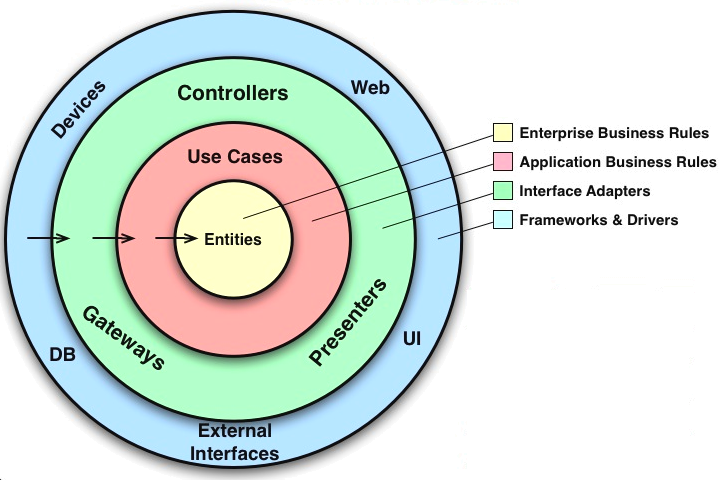
\includegraphics[width=\textwidth,keepaspectratio=true]{contextualizacion/MarcoReferencial/imgs/clean_architecture.png}%
\caption{Arquitectura Limpia.} \label{fig:clean_architecture}
\end{figure}


La propuesta del Tío Bob sobre la arquitectura limpia impone las siguientes restricciones:\\

\begin{itemize}
\item \textbf{Independiente de frameworks:} la arquitectura no debe atarse a las restricciones del framework. Esto permite considerar al framework como una herramienta.
\item \textbf{Testeable:} las reglas de negocios deberían poder probarse independientemente de la UI, base de datos u otras herramientas.
\item \textbf{Independiente de la UI:} la interfaz de usuario se debería poder cambiar fácilmente sin necesidad de cambiar la lógica de negocio.
\item \textbf{Independiente de la base de datos:} las reglas de negocios no deberían estar ligadas a la base de datos o herramienta de persistencia.
\end{itemize}

\subsubsection{\textbf{MVP}}
Es una derivación del patrón arquitectónico modelo–vista–controlador (MVC), y es utilizado mayoritariamente para construir interfaces de usuario\\
En MVP el presentador asume la funcionalidad del "intermediario". En MVP, toda lógica de presentación es colocada al presentador \citeW{mvp_2018}.\\
MVP es un patrón arquitectónico de interfaz de usuario diseñada para facilitar pruebas de unidad automatizada y mejorar la separación de inquietudes en lógica de presentación:
\begin{itemize}
\item El modelo es una interfaz que define los datos que se mostrarán o no actuado en la interfaz de usuario.
\item El presentador actúa sobre el modelo y la vista. Recupera datos de los repositorios (el modelo), y los formatea para mostrarlos en la vista.
\item La vista es una interfaz pasiva que exhibe datos (el modelo) y órdenes de usuario de las rutas (eventos) al presentador para actuar sobre los datos.
\end{itemize}

\subsubsection{\textbf{SISTEMAS DE RECOMENDACIÓN}}
Es un sistema inteligente que proporciona a los usuario sugerencias personalizadas sobre un determinado tema. Estudian el perfil del cliente, sus búsquedas anteriores, sus compras, perfiles, páginas visitadas, recopilan toda esta información e intentan hace sugerencias que son de interés del usuario.\\

Uno de los sistemas de recomendación famosos son, Amazon e Youtube, la primera utiliza la información de las compras de los usuarios, la navegación y búsqueda de los productos para sugerir posibles productos de interés. Youtube registra la búsqueda de vídeos y la visualización de vídeos para mostrar sugerencias de vídeos que le podrían gustar.
\citeW{Quesonl99:online}

Los sistemas de clasificación se pueden dividir en 4 tipos:  

\begin{enumerate}
\item \textbf{Filtrado basado en Contenido} Las recomendaciones se basan en el conocimiento que se tiene sobre los items que el usuario ha valorado (ya sea de forma implícita o explícita), y se le recomendarán items similares que le puedan gustar o interesar. Un ejemplo de es Youtube.
\item  \textbf{Filtrado Demográfico:} Estas recomendaciones se realizan en función de las características de los usuarios (edad, sexo, situación geográfica, profesión, etc).
\item \textbf{Filtrado Colaborativo:} Consiste en ver que usuarios son similares al usuario activo (o usuario al que hay que realizarle las recomendaciones) y a continuación,recomendar aquellos items que no han sido votados por el usuario activo y que han resultado bien valorados por los usuarios similares. Un ejemplo de es Filmaffinity.
\item \textbf{Filtrado Híbrido}:  Mezclan alguno de los tres filtrados mencionados anteriormente para realizar recomendaciones e incluso lo combinan con alguna otra técnica de inteligencia artificial como pueda ser la lógica borrosa o la computación evolutiva. Un ejemplo es Amazon.
\end{enumerate}


\begin{figure}[htbp]
\centering%
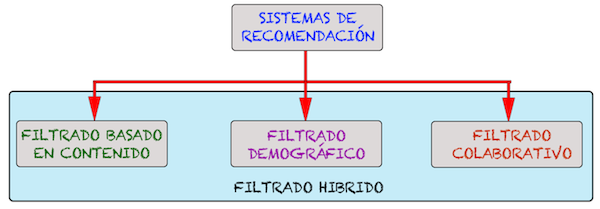
\includegraphics[width=\textwidth,keepaspectratio=true]{contextualizacion/MarcoReferencial/imgs/Sistema-de-Recomendacion-Clasificacion-jarroba.png}%
\caption{Tipos de sistema de recomendación. \citeW{Quesonl99:online}} \label{fig:sisrec}
\end{figure}

\subsubsection{\textbf{MICROSERVICIOS}}
Se define un microservicio es una pequeña aplicación que puede ser desplegada, probada y escalada de forma independiente y que tiene una única responsabilidad\cite{7030212}. Hablamos de única responsabilidad en su definición básica, que es que solo se tenga que cambiar por sola una cosa \cite{Martin:2008:CCH:1388398}.

\subsubsubsection{\textbf{\textit{¿Qué se debe tener en cuenta?}}}

Se espera que un microservicios no tengo muchas líneas de código y puedas entrar todo su poder a sólo una funcionalidad. Normalmente cuando se empieza en un proyecto, se inicia con una aplicación monolítica, que para un inicio están bien, pero a medida que el proyecto va creciendo se vuelve más complicado su mantenibilidad, su escalabilidad, sus pruebas debido a que todos los proyectos los servicios están unidos, haciendo que los despliegues se vuelvan complicados y muy grandes. Al tener una aplicación monolítica, hace que un fallo en uno de los servicios puede tumbar toda nuestra aplicación, una cosa que no deseamos. Y también si queremos hacer un pequeño cambio en nuestro código significa que tenemos que desplegar toda la aplicación, no se puede desplegar sobre el pequeño cambio que hicimos. Estos son unos de los problemas que intenta atacar la arquitectura por microservicios, y por lo cuál en los últimos tiempos se han vuelto tan utilizada, haciendo servicios compactos e independientes hacemos que se pueda tomar ventaja de todas las tecnologías que hay en el mercado pudiendo a cada uno de los servicios especializarlo en la tecnología que más le convenga, estos servicios son especializados, o sea que sólo tienen una una responsabilidad lo cual los hace fácil de escalar de mantener y de probar. Un módulo común de esta arquitectura es que tenga la lógica de negocio asociado con la base de datos la base de datos Y es única para ese servicio, esto implica que si queremos hacer un cambio en ese servicio sólo tenemos que desplegar ese servicio sin afectar los demás, asimismo, si un servicio falla todos los otros servicios de nuestra aplicación pueden seguir funcionando.

\subsubsubsection{\textbf{\textit{¿Es buena idea iniciar de una con microservicios?}}}

Cuando se decide implementar una arquitectura por microservicios debe tener muy claro la lógica del negocio, porque hay que saber muy bien cómo se va a dividir el proyecto en los diferentes servicios, en cada uno de los servicios para así no tener problemas más adelante, la mayoría de empresas que han implementado microservicios, lo primero que han tenido es una aplicación monolítica, una aplicación con todos sus servicios integrados y a medida que van creciendo y ya con la lógica de negocio clara, definen los servicios que necesitan y empiezan a dividir su código monolítico en servicios más pequeños y especializados \cite{Dragoni2017}. 

\subsubsubsection{\textbf{\textit{¿Es compleja la migración?}}}

La respuesta concisa es que si, al tener muchos microservicios empezamos a tener necesidades que no teníamos antes con las aplicaciones monolíticas, tenemos que tener en cuenta que pueden ser muchos servicios que se van a estar comunicando entre ellos y hacia el exterior, aquí es donde nos empieza a apoyar todas las herramientas de despliegue continuo y computación en la nube, al tener muchos servicios nos encontramos con el inconveniente de tener que hacer muchos despliegues y muchas configuraciones en ambientes separados lo cual sin herramientas que nos ayuden a esta tarea sería muy complicado de mantener, adicionalmente pensando en la escalabilidad de un sistema nos damos cuenta de que esos servicios se pueden duplicar, triplicar, ...,  dependiendo de la carga dependiendo lo que de las configuraciones que tengamos, lo cual hace que no podemos tener direcciones o apuntador servicios estáticos, tenemos que tener herramientas o servicios que nos permitan dinámicamente encontrar todos los microservicios de nuestra aplicación, con esto queremos decir que una aplicación de microservicios no es sólo dividir servicios y ya, detrás de eso tenemos lógicas esenciales y herramientas para que esto pueda funcionar la forma correcta y que no se nos vuelva un problema al final. Para esto vamos a utilizar toda la parte de integración continua y adicionalmente servicios de Gateway que nos permitan encontrar y distribuir nuestros servicios \citeW{Microser11:online}\cite{Dragoni2017}.

\subsection{Marco Legal}
\subsubsection{Papel del estado y las instituciones públicas }
Al Estado le corresponde:\\

Promover y fomentar el acceso a la cultura de todos los colombianos en igualdad de
oportunidades, por medio de la educación permanente y la enseñanza científica,
técnica, artística y profesional; Promover la investigación la ciencia, el desarrollo y la
difusión de los valores culturales de la nación (Art 70. Constitución Política)\\

Crear incentivos para personas e instituciones que desarrollen y fomenten la ciencia y
la tecnología y las demás manifestaciones culturales y ofrecer estímulos a quienes
ejerzan estas actividades. (Artículo 71. Constitución Política).\\

Impulsar y estimular los procesos, proyectos y actividades culturales en un marco de
reconocimiento y respeto por la diversidad. (Articulo 1-3, ley 397 de 1997)\\

Abstenerse de ejercer censura sobre la forma y el contenido ideológico y artístico de
las realizaciones culturales y proyectos culturales (Art, 1-4, ley 397 de 1997) \\

Promover la interacción de la cultura nacional con la cultura universal (Art, 1-12, ley
397 de 1997)\\

Garantizar el acceso de los colombianos a las manifestaciones, bienes y servicios
culturales. (Art, 1-13, ley 397 de 1997) \citeW{bernal_2018}

\section{Aspectos metodológicos}
\subsection{Tipo de estudio}
El tipo de investigación utilizado en la generación de este prototipo será proyectiva/interactiva\cite{holistica}. lo anterior teniendo en cuenta que la idea central del proyecto es proponer una nueva forma de realizar un proceso de contratación que modifique la que en este momento se utiliza de manera común, mejorandola y proyectándola a posiblemente impulsar nuevos talentos y apoyarlos en procesos administrativos y de negocios a los que no están acostumbrados comportándose como un manager para artistas informales que de pronto no cuenten con los recursos necesarios para adquirir dichos servicios.
\subsection{Método de investigación}
Para lograr el fin deseado utilizaremos apartes de cada uno de los niveles de la investigación holística de la siguiente manera:

\textbf{Perceptual}: Exploraremos las opciones utilizadas en la actualidad para lograr la contratación de un servicio de entretenimiento; describiéndolo de manera que encontremos sus falencias y oportunidades de mejora.

\textbf{Aprehensivo}: Compararemos las formas en las que se realiza el proceso de selección de artistas informales y analizaremos la que produzca mayor impacto para extraer de hay los puntos fuertes que deben incluirse en nuestra propuesta.

\textbf{Comprensivo}: Propondremos una nueva opción que cubra las necesidades de veladas en los pasos anteriores.

\textbf{Integrativo}: Apuntaremos a modificar la forma en que se realiza el proceso de selección al momento de elegir un artista informal para una presentación  

\subsection{Fuentes y técnicas para la recolección de la información}
La información primaria se obtendrá de la aplicación de una encuesta que determine la forma de contratación de servicios artísticos en una población controlada mayor de edad que esté en la capacidad de realizar dicho proceso, se generan preguntas cerradas que limitan las posibilidades de existentes y describan el proceso actual y la opción de cambiarlo.\\

Como segunda fuente se verificarán las bases de datos científicas especializadas en ingeniería para aplicar las metodologías necesarias en cuanto a la producción de software de calidad y que den valor agregado al producto final enmarcadas en procesos conocidos y de trazabilidad comprobable. Además de las generalidades legales y sociales que pueda acarrear el uso de material multimedia con propiedad intelectual. 

\subsection{Tratamiento de la información}

La información recopilada a través de la aplicación de la encuesta será anónima sin causar perjuicio a los originadores de la misma. Luego de ser obtenida se analizará para seleccionar las coincidencias importantes y generar las directrices de modelamiento del producto de software que se planea construir. 
Por otro lado la documentación técnica guía para el desarrollo del software será claramente referenciada en la bibliografía del producto dando el valor a las mismas y respetando los principios de propiedad intelectual.

\section{Organización del trabajo de grado}
%\chapter{Estudio Sistemas previos}
%\begin{appendix}
\chapter{Anexo: Nombrar el anexo A de acuerdo con su contenido}\label{AnexoA}
Los Anexos son documentos o elementos que complementan el cuerpo de la tesis o trabajo de investigaci\'{o}n y que se relacionan, directa o indirectamente, con la investigaci\'{o}n, tales como acetatos, cd, normas, etc.\\

\chapter{Anexo: Nombrar el anexo B de acuerdo con su contenido}
A final del documento es opcional incluir \'{\i}ndices o glosarios. \'{E}stos son listas detalladas y especializadas de los t\'{e}rminos, nombres, autores, temas, etc., que aparecen en el mismo. Sirven para facilitar su localizaci\'{o}n en el texto. Los \'{\i}ndices pueden ser alfab\'{e}ticos, cronol\'{o}gicos, num\'{e}ricos, anal\'{\i}ticos, entre otros. Luego de cada palabra, t\'{e}rmino, etc., se pone coma y el n\'{u}mero de la p\'{a}gina donde aparece esta informaci\'{o}n.\\

\chapter{Anexo: Nombrar el anexo C de acuerdo con su contenido}
MANEJO DE LA BIBLIOGRAF\'{I}A: la bibliograf\'{\i}a es la relaci\'{o}n de las fuentes documentales consultadas por el investigador para sustentar sus trabajos. Su inclusi\'{o}n es obligatoria en todo trabajo de investigaci\'{o}n. Cada referencia bibliogr\'{a}fica se inicia contra el margen izquierdo.\\

La NTC 5613 establece los requisitos para la presentaci\'{o}n de referencias bibliogr\'{a}ficas citas y notas de pie de p\'{a}gina. Sin embargo, se tiene la libertad de usar cualquier norma bibliogr\'{a}fica de acuerdo con lo acostumbrado por cada disciplina del conocimiento. En esta medida es necesario que la norma seleccionada se aplique con rigurosidad.\\

Es necesario tener en cuenta que la norma ISO 690:1987 (en Espa\~{n}a, UNE 50-104-94) es el marco internacional que da las pautas m\'{\i}nimas para las citas bibliogr\'{a}ficas de documentos impresos y publicados. A continuaci\'{o}n se lista algunas instituciones que brindan par\'{a}metros para el manejo de las referencias bibliogr\'{a}ficas:\\

\begin{center}
\centering%
\begin{tabular}{|p {7.5 cm}|p {7.5 cm}|}\hline
\arr{Instituci\'{o}n}&Disciplina de aplicaci\'{o}n\\\hline%
Modern Language Association (MLA)&Literatura, artes y humanidades\\\hline%
American Psychological Association (APA)&Ambito de la salud (psicolog\'{\i}a, medicina) y en general en todas las ciencias sociales\\\hline
Universidad de Chicago/Turabian &Periodismo, historia y humanidades.\\\hline
AMA (Asociaci\'{o}n M\'{e}dica de los Estados Unidos)&Ambito de la salud (psicolog\'{\i}a, medicina)\\\hline
Vancouver &Todas las disciplinas\\\hline
Council of Science Editors (CSE)&En la actualidad abarca diversas ciencias\\\hline
National Library of Medicine (NLM) (Biblioteca Nacional de Medicina)&En el \'{a}mbito m\'{e}dico y, por extensi\'{o}n, en ciencias.\\\hline
Harvard System of Referencing Guide &Todas las disciplinas\\\hline
JabRef y KBibTeX &Todas las disciplinas\\\hline
\end{tabular}
\end{center}

Para incluir las referencias dentro del texto y realizar lista de la bibliograf\'{\i}a en la respectiva secci\'{o}n, puede utilizar las herramientas que Latex suministra o, revisar el instructivo desarrollado por el Sistema de Bibliotecas de la Universidad Nacional de Colombia\footnote{Ver: www.sinab.unal.edu.co}, disponible en la secci\'{o}n "Servicios", opci\'{o}n "Tr\'{a}mites" y enlace "Entrega de tesis".

\end{appendix}

\part{DESARROLLO DE LA INVESTIGACIÓN}

\chapter{Recolección y ordenamiento de la información}
\section{Encuesta}
La herramienta presentada a continuación se realizo en la plataforma Formularios de Google, teniendo en cuenta que el producto planteado es una solución tecnológica y por lo tanto la muestra debería por supuesto tener acceso a la tecnología y ser mayores de edad, con estas dos únicas restricciones se aplico la siguiente encuesta\\
\\
\begin{enumerate}
\item ¿Alguna vez he contratado un servicio de músicos informales?
\item  ¿En el futuro planeo utilizar algún servicio de músicos informales?
\item  ¿Conozco algún artista que necesite promoción?
\item  ¿Conozco alguna plataforma o aplicación de contratación de servicios de músicos informales?
\item  Si la respuesta anterior fue sí, escriba cuál
\item  ¿Utilizó alguna plataforma o aplicación de música o entretenimiento y la tengo configurada a mi gusto?
\item  Si la respuesta anterior fue sí, escriba cual
\item  Cuando contrato un músico informal, me gusta:
    \begin{enumerate}
    \item Contratarlo personalmente
    \item Ver presentaciones anteriores
    \item Saber el costo del servicio
    \item Solo con una recomendación es suficiente
    \item Leer comentarios
    \item Pagar por el servicio en efectivo
    \item Pagar por el servicio con tarjeta
    \end{enumerate}
\item  Si pudiera ver comentarios, vídeos, imágenes y calificación de un grupo o músico informal, ¿lo contrataría a través de una plataforma digital?
    \begin{enumerate}
    \item si
    \item no
    \end{enumerate}
\item  Si la respuesta anterior fue no, escriba las razones
\item  ¿Con qué frecuencia ud. contrata músicos informales para sus eventos?
    \begin{enumerate}
    \item una vez al mes
    \item una vez por trimestre
    \item una vez por semestre
    \item una vez por año
    \item casi nunca
    \end{enumerate}
\end{enumerate}
\section{Tabulación y ordenamiento de información}

\begin{center}
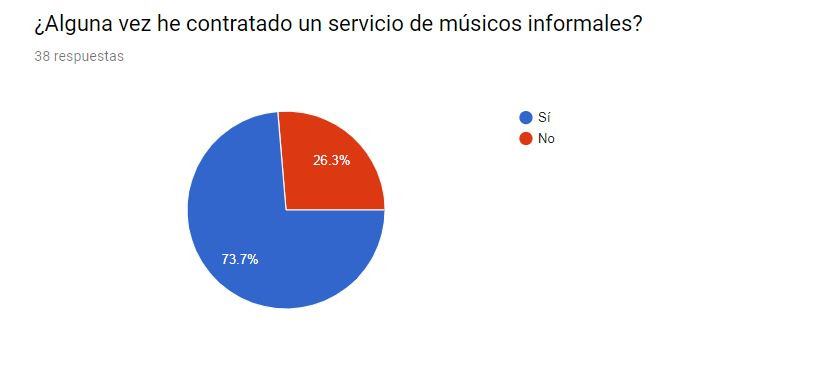
\includegraphics[width=16cm, height=10cm,keepaspectratio=true]{Desarrollo/RecoleccionInformacion/imgs/1.JPG}
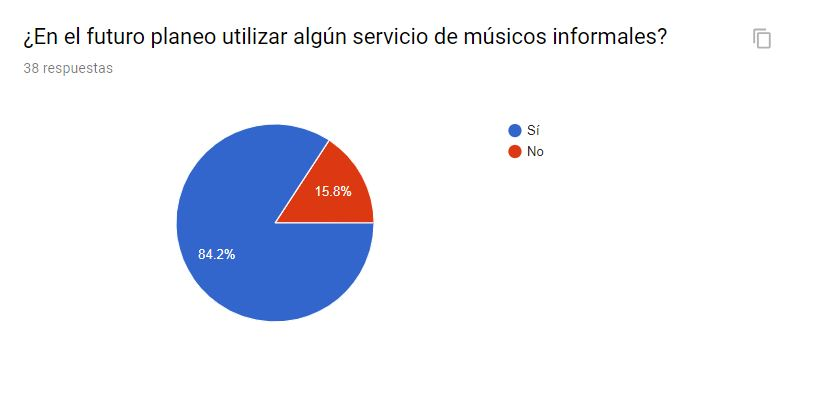
\includegraphics[width=16cm, height=10cm,keepaspectratio=true]{Desarrollo/RecoleccionInformacion/imgs/2.JPG}
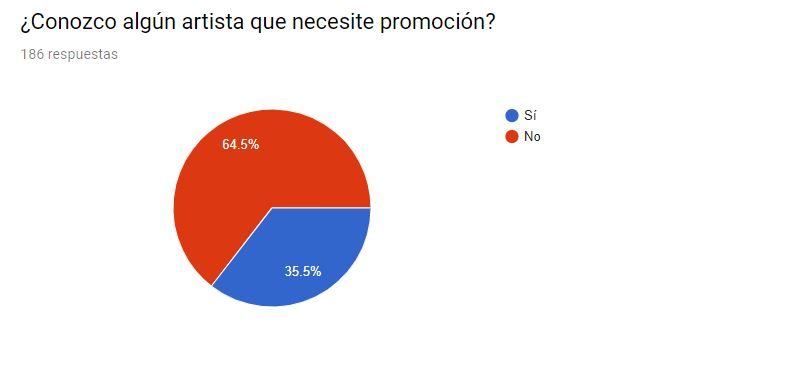
\includegraphics[width=16cm, height=10cm,keepaspectratio=true]{Desarrollo/RecoleccionInformacion/imgs/3.JPG}
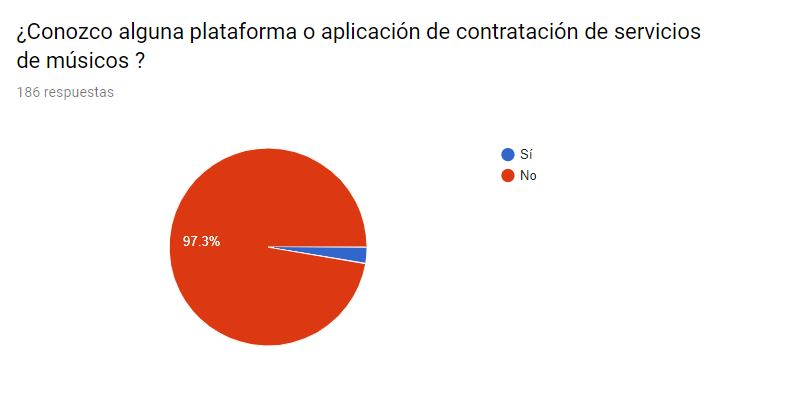
\includegraphics[width=16cm, height=10cm,keepaspectratio=true]{Desarrollo/RecoleccionInformacion/imgs/4.JPG}

\includegraphics[width=16cm, height=10cm,keepaspectratio=true]{Desarrollo/RecoleccionInformacion/imgs/5.JPG}
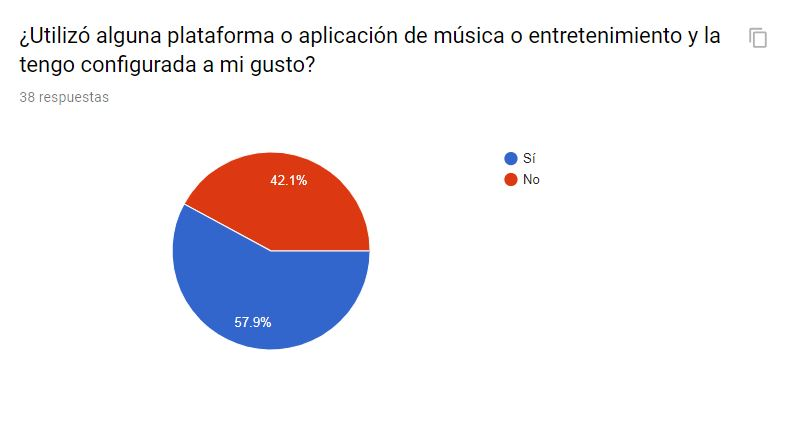
\includegraphics[width=16cm, height=10cm,keepaspectratio=true]{Desarrollo/RecoleccionInformacion/imgs/6.JPG}
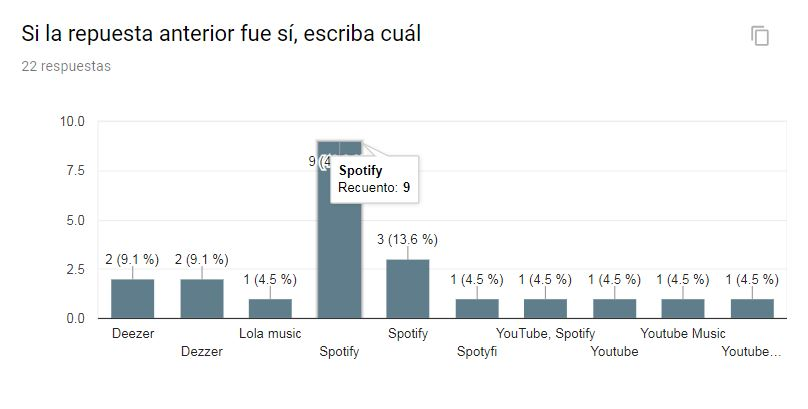
\includegraphics[width=16cm, height=10cm,keepaspectratio=true]{Desarrollo/RecoleccionInformacion/imgs/7.JPG}
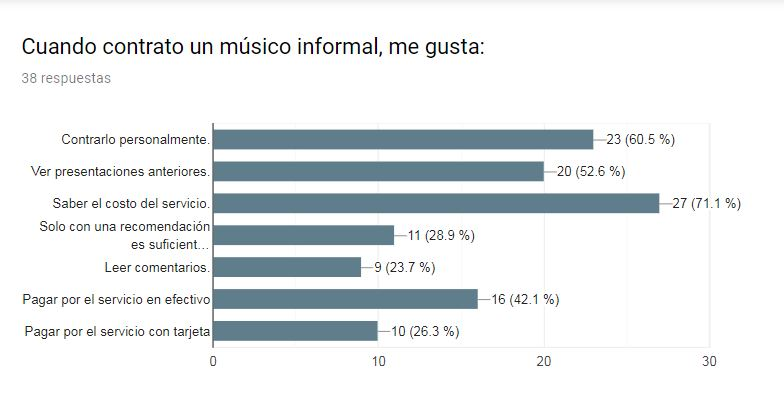
\includegraphics[width=16cm, height=10cm,keepaspectratio=true]{Desarrollo/RecoleccionInformacion/imgs/8.JPG}
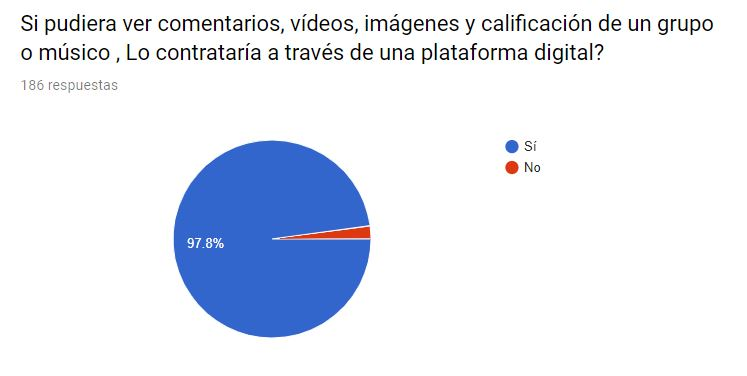
\includegraphics[width=16cm, height=10cm,keepaspectratio=true]{Desarrollo/RecoleccionInformacion/imgs/9.JPG}
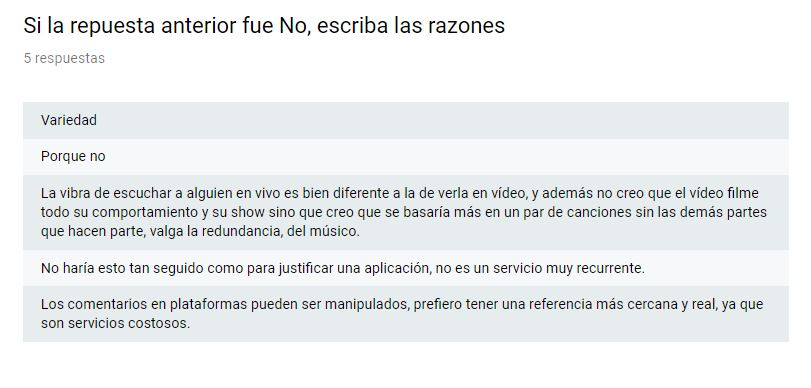
\includegraphics[width=16cm, height=10cm,keepaspectratio=true]{Desarrollo/RecoleccionInformacion/imgs/10.JPG}
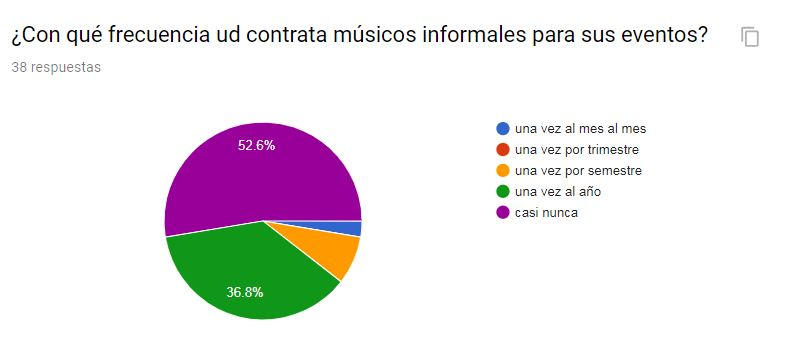
\includegraphics[width=16cm, height=10cm,keepaspectratio=true]{Desarrollo/RecoleccionInformacion/imgs/11.JPG}
\end{center}

\newpage
\section{Análisis de la información}

La muestra tuvo un tamaño de 186 individuos que aplicando la siguiente ecuación:
\begin{center}
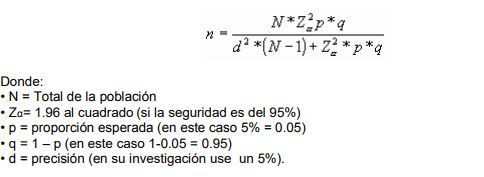
\includegraphics[width=16cm, height=10cm,keepaspectratio=true]{Desarrollo/RecoleccionInformacion/imgs/muestra.JPG}
\end{center}
Nos genera la siguiente relación:\\ 
Para una población de (4.550.000) adultos mayores de 18 años en Bogota, con un porcentaje de 95\% de precision y un 7.3 \%  de error  se necesitarían 184 individuos, de esta manera cumplimos con el mínimo solicitado.\\
Estos 186 individuos clasifican en los siguientes grupos:\\
\begin{center}
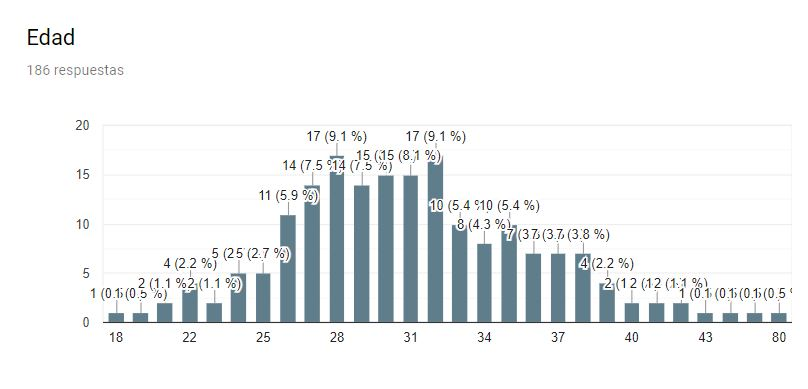
\includegraphics[width=16cm, height=10cm,keepaspectratio=true]{Desarrollo/RecoleccionInformacion/imgs/edad.JPG}
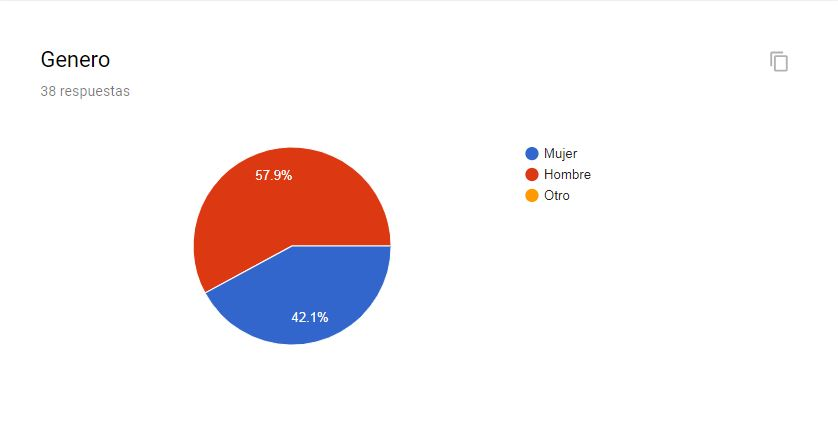
\includegraphics[width=16cm, height=10cm,keepaspectratio=true]{Desarrollo/RecoleccionInformacion/imgs/genero.JPG}
\end{center}
De lo anterior se infiere la viabilidad del proyecto; pues de una muestra variada y posibilitada para utilizarlo, presenta una expectativa de consumo del 97.8 \% \\
Por otro lado el consumo del servicio seria apropiado teniendo en cuenta que para una muestra de este tamaño el 69.9 \% utilizara los servicios de un músico informal. Y aunque el 62.9 \% dijo nunca realizar esta actividad se pueden interesar por la reproducción y visualización de medios multimedia como entretenimiento.\\
Se evidencio que en el futuro cercano si existe la posibilidad de realizar la contratación de un musico informal; pero la dificultad o la falta de conocimiento en el proceso disminuye el interés, por lo que la solución planteada debe ser lo mas simple y sencilla y por otro lado como el procedimiento centralizara todo la transcendida se espera gran acogida.


\chapter{Fases del diseño del prototipo}
\section{Arquitectura Empresarial}
\subsection{Aplicación}
\subsection{Infraestructura}
\subsection{Motivacional}
\section{Historias de usuario}
\section{Modelo de datos}
\begin{figure}[htbp]
\centering%M
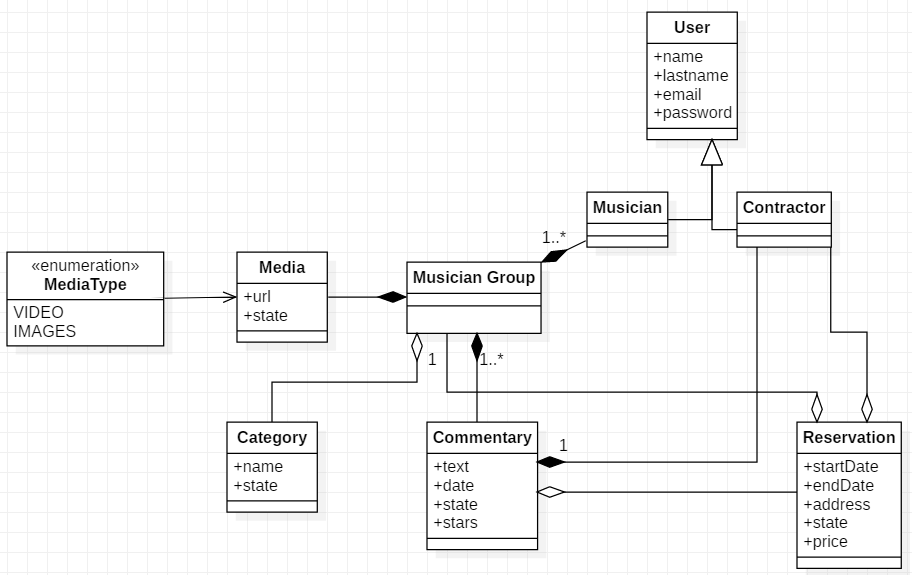
\includegraphics[width=\textwidth,keepaspectratio=true]{Desarrollo/ModeloDatos/imgs/Clases.PNG}%
\caption{Modelo de datos.} \label{fig:modeldata}
\end{figure}
\section{Interfaces de usuario}
A continuación se realiza la presentación del demo que se espera del producto final.
\subsection{Iniciar Sesión:}

\begin{figure}[h!]
 \centering
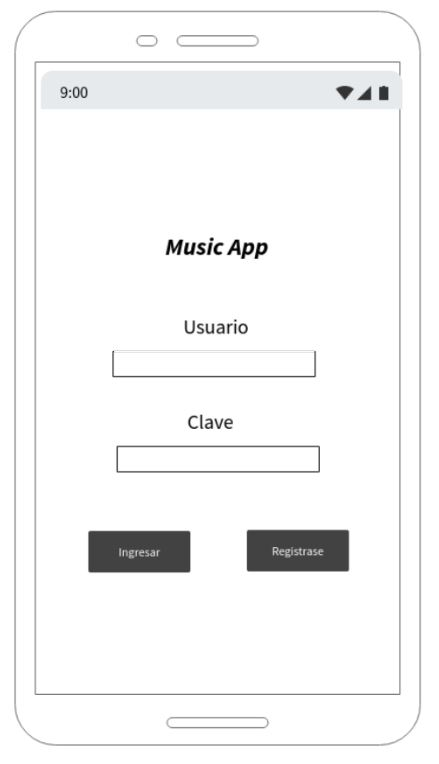
\includegraphics[width=12cm, height=16cm,keepaspectratio=true]{Desarrollo/Interfaces/imgs/wire1.JPG}
\end{figure}
\newpage
\subsection{Registrar nueva cuenta:}

\begin{figure}[h!]
 \centering
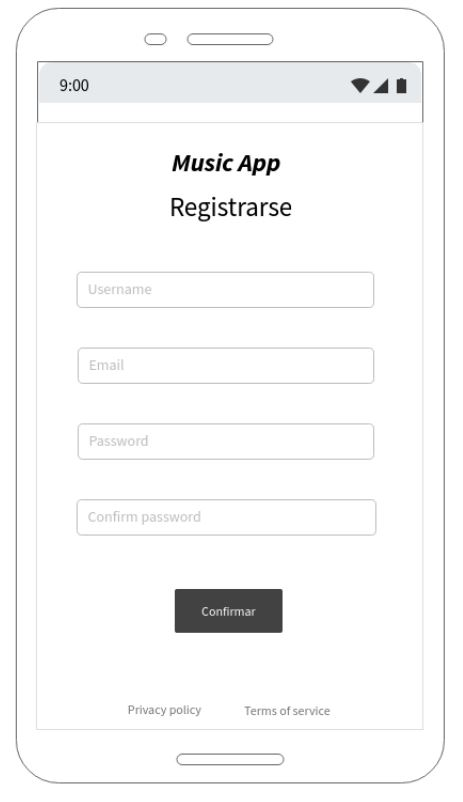
\includegraphics[width=12cm, height=16cm,keepaspectratio=true]{Desarrollo/Interfaces/imgs/wire2.JPG}
\end{figure}
\newpage
\subsection{Visualización ofertas:}

\begin{figure}[hbt!]
 \centering
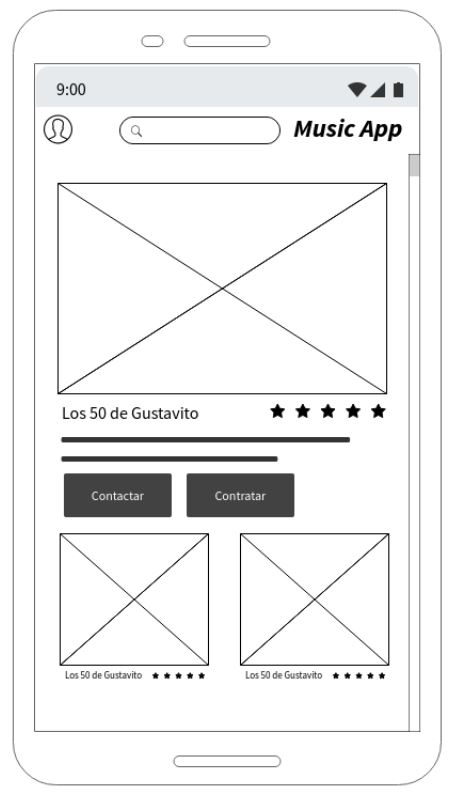
\includegraphics[width=12cm, height=16cm,keepaspectratio=true]{Desarrollo/Interfaces/imgs/wire3.JPG}
\end{figure}
\newpage
\subsection{Contactar:}

\begin{figure}[hbt!]
 \centering
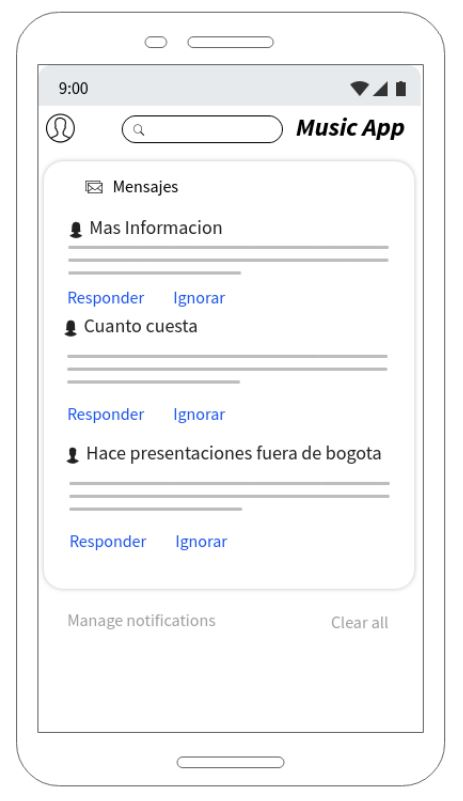
\includegraphics[width=12cm, height=16cm,keepaspectratio=true]{Desarrollo/Interfaces/imgs/wire4.JPG}
\end{figure}
\newpage
\subsection{Agenda de servicios:}

\begin{figure}[hbt!]
 \centering
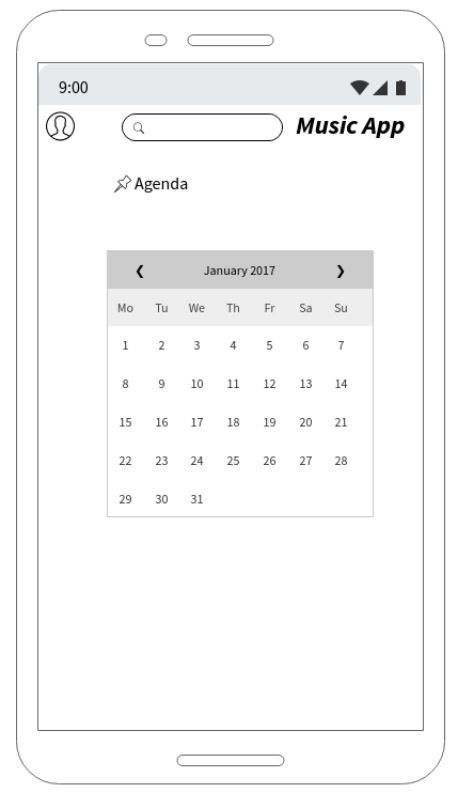
\includegraphics[width=12cm, height=16cm,keepaspectratio=true]{Desarrollo/Interfaces/imgs/wire5.JPG}
\end{figure}
\newpage
\subsection{Contratos realizados:}

\begin{figure}[hbt!]
 \centering
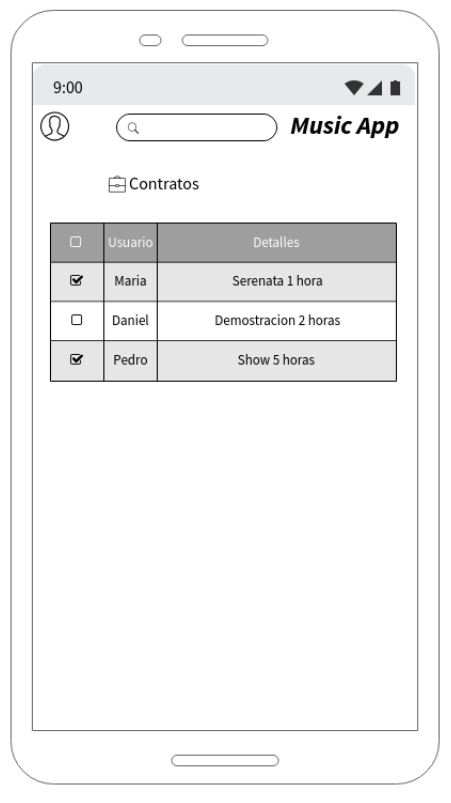
\includegraphics[width=12cm, height=16cm,keepaspectratio=true]{Desarrollo/Interfaces/imgs/wire6.JPG}
\end{figure}
\newpage
\subsection{Calificar servicio:}

\begin{figure}[hbt!]
 \centering
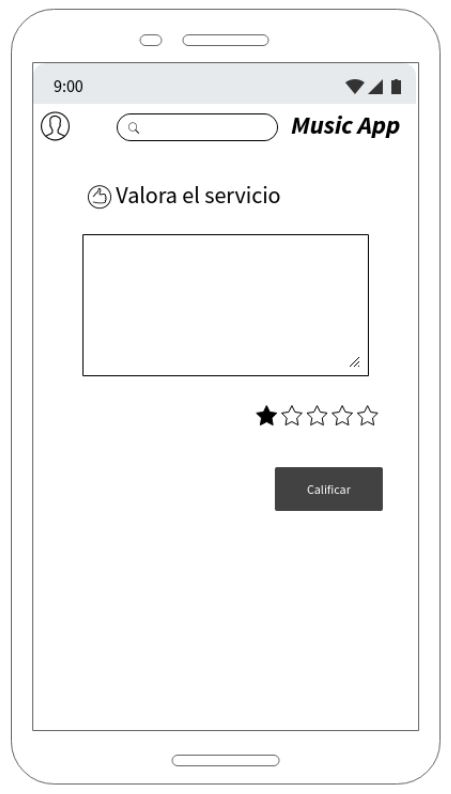
\includegraphics[width=12cm, height=16cm,keepaspectratio=true]{Desarrollo/Interfaces/imgs/wire7.JPG}
\end{figure}

\chapter{Desarrollo de funcionalidades del prototipo}

\part{ CIERRE DEL PROYECTO}
\chapter{Resultados}
\chapter{Conclusiones}
\chapter{Prospectiva del trabajo de grado}
\chapter{Líneas de investigación futuras}
\chapter{Trabajos de Investigación futuros}

\addcontentsline{toc}{chapter}{Bibliografía}
\bibliographystyle{plaindin_esp}
\bibliography{Bibliografia/biblo}

\addcontentsline{toc}{chapter}{Referencias Web}
\bibliographystyleW{plaindin_esp}
\bibliographyW{Bibliografia/web}

%\addcontentsline{toc}{chapter}{\numberline{}Bibliograf\'{\i}a}
%\bibliographystyle{plaindin_esp}
%\bibliography{biblo}
\end{document}